\documentclass{article}

\usepackage{repsty}
\usepackage{wrapfig}

\usepgfplotslibrary{fillbetween}


\begin{document}
	
\section*{Problem statement}

Our goal is to estimate the frequency $\omega$ of the signal
\begin{equation}
	N(t) = N_0\cdot\bkt{1 + P\cdot e^{-\sfrac{t}{\tau_d}}\cdot\sin(\omega\cdot t + \phi)},
\end{equation}
where $\tau_d$ is the spin tune lifetime. One observation $N_i = N(t_i)$ takes anywhere between 1--10 milliseconds, and involves two to three thousands of polarimetry measurements.

Assuming the Normal error distribution with mean zero and variance $\nu = \SD{\obs}^2$, the maximum likelihood estimator for the variance of the frequency estimate can be expressed as
\begin{equation}\label{eq:SEFreqEst}
\begin{cases}
\var{\hat\omega} &= \nu\bkt{\sum_j x_j\cdot \var[w]{t}}^{-1}, \\
\var[w]{t} &= \sum_i w_i \bkt{t_i - \avg{t}_w}^2,~ \avg{t}_w = \sum_i t_i w_i, \\
w_i &= \frac{x_i}{\sum_j x_j},~ x_i = (N_0P\exp(\lambda t_i))^2\cos^2(\omega t_i + \phi) = \bkt{\mupp}^2.
\end{cases}	
\end{equation}
As expected, the variance is inversely proportional to the (weighted) spread of the predictor variable,
% times the normalizing constant that is a measure of the sample's informational content, 
and directly proportional to the variance of the error. 

Regarding the former, the weighting by the derivative of the signal has a twofold effect: in the first place, observations that are made when the derivative is maximal to the spread more than those made when the signal changes slowly. Considering the number of possible observations during a fill is limited, a more cost-effective use of the beam is a concern; one that could be addressed by sampling only during the periods of rapid change in the signal. In the second place, due to spin tune decoherence, the observations' contribution goes down with time. This aspect restricts our ability to maximize sampling efficiency. A possible trade-off would be to reduce the number of polarimetry measurements involved in, and thus the time of, making an observation. That way, more observations could be squeezed in the periods when the sine changes sign (zero-crossings), but simultaneously, the uncertainty of an observation would be increased. 

The above considerations prompt the following series of questions:
\begin{enumerate}
	\item How long to measure the signal?
	\item How many measurements per observation are optimal?
	\item How congregated about the zero-crossings the measurements should be?
\end{enumerate}
We will try to answer them in what follows.

\section{Number of measurements per observation (event)}

Define the following variables: \begin{inparaenum}[\itshape a\upshape)]
	\item the number of measurements per observation: $\Nmo$;
	\item the number of observations per zero-crossing: $\Nozc$;
	\item the number of zero-crossings per experiment: $\Nzc$.
\end{inparaenum}

The expected total number of scatterings in an experiment with a given number of zero-crossings: $n_m = \underbrace{\Nzc\cdot\Nozc}_{\No}\cdot\Nmo$. ($\No$ is the total number of observations.)

\begin{equation}
\begin{cases}
	\SE{\hat{\omega}}^2 &= \frac{\SD{\obs}^2}{X_{tot}\cdot\sum_{j=1}^{\No}w_j\bkt{t_j - \avg{t}_w}^2}, \\
	\SE{\obs}^2 &= \frac{\SD{\meas}^2}{\Nmo} ,\\
	X_{tot} &= \sum_{j=1}^{\No} x_j = \sum_{s=1}^{\Nzc}\sum_{j=1}^{\Nozc} x_{js}.
\end{cases}
\end{equation}

We can express $\sum_{j=1}^{\Nozc} x_{js} = \Nozc \cdot x_{0s}$, for some mean value $x_{0s}$ in the given zero-crossing $s$. The sum $\sum_{j=1}^{\Nozc} x_{js}$ falls exponentially due to decoherence, hence $x_{0s} = x_{01}\exp{(\lambda\cdot \frac{(s-1)\cdot\pi}{\omega})}$. Therefore,
\[
	X_{tot} = \Nozc\cdot x_{01} \cdot \frac{\exp{\bkt{\frac{\lambda\pi}{\omega}\Nzc}}-1}{\exp{\bkt{\frac{\lambda\pi}{\omega}}}-1} \equiv \Nozc \cdot g(\Nzc).
\]

\begin{figure}[h]
	\centering
	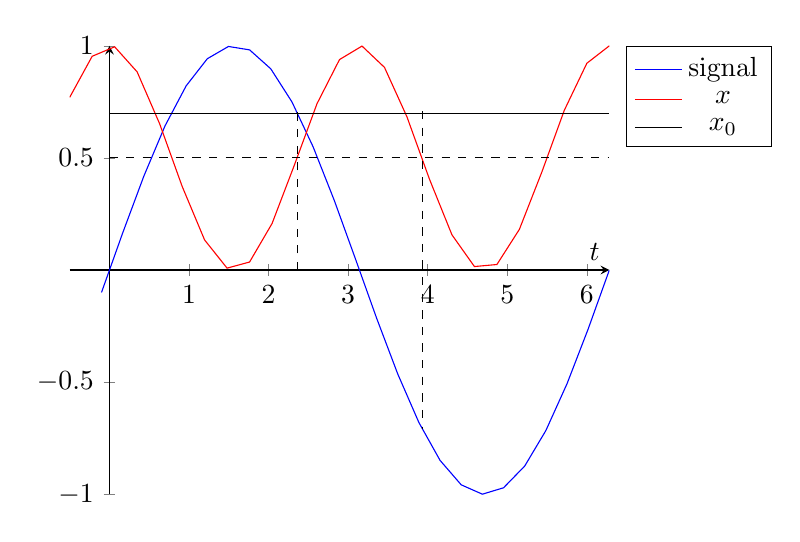
\begin{tikzpicture}
		\begin{axis}[axis lines=center, xlabel=$t$, domain=-.5:2*pi, legend pos=outer north east]
		\addplot[color=blue, name path=signal, domain=-.1:2*pi] {sin(deg(x))}; \addlegendentry{signal}
		\addplot[color=red] {cos(deg(x))^2}; \addlegendentry{$x$}
		\addplot[mark=none, domain=0:2*pi]{.7}; \addlegendentry{$x_0$}
		\addplot[mark=none,dashed, domain=0:2*pi]{.5};
		\draw[dashed] (axis cs:2.36,0) -- (axis cs:2.36,{sin(deg(2.36))});
		\draw[dashed] (axis cs:3.93,{-sin(deg(3.93))}) -- (axis cs:3.93,{sin(deg(3.93))});
		\end{axis}
	\end{tikzpicture}
	\caption{Explanation for $x_0$\label{fig:x0Expl}}
\end{figure}

The number of events per zero-crossing 
\[
	\Nozc = \frac{\Delta t_{zc}}{\Nmo\cdot \Delta t_{\meas}},
\]
hence
\[
	X_{tot} = g(\Nzc) \cdot \frac{\Delta t_{zc}}{\Delta t_{\meas}}\cdot \frac{1}{\Nmo}.
\]

The variance $\var[w]{t}$ is also practically independent of how many measurements there are per one zero-crossing (and by extension, the number $\Nmo$), and depends primarily on the $\Nzc$ and decoherence life time.

In sum, assuming one observation is the mean of the measurements ($\SD{\obs} = \SD{\meas}/\sqrt{\Nmo}$), 
\begin{align*}
	\var[w]{\hat{\omega}} &= \frac{\SD{\meas}^2\cdot \sfrac{1}{\Nmo}}{g(\Nzc)\cdot \frac{\Delta t_{zc}}{\Delta t_{\meas}}\cdot \sfrac{1}{\Nmo} \cdot \var[w]{t}} \\
		&= \frac{\SD{\meas}^2}{g(\Nzc)\cdot \frac{\Delta t_{zc}}{\Delta t_{\meas}} \cdot \var[w]{t}}.
\end{align*}
There's no benefit to increasing the number of measurements per observation.

\section{Modulation}

In order to increase beam use efficiency, it is advantageous to sample the signal only during rapid change. That way, the yield of Fisher information per scattered particle is maximized. However, one has to take into account that the beam polarization dissipates continuously, whether the beam is being sampled or not, and so there's a finite window in which sampling yields statistically significant results. We will estimate how long that is in the next section, but for now we will assume that it is less than the beam lifetime when it is scattered continuously.

Then frequency-modulated sampling will perform worse than uniform sampling. That is because, unless observations are made proportionally faster, there will be fewer points sampled by the time the signal is indistinguishable from noise. But an increase in sampling frequency would not have any effect on the result, because observation variance is increased proportionally.


\section{Spin tune decoherence time}

A rough estimate of the maximum sensible experiment duration could be done by considering the time when the signal oscillation is indistinguishable from noise. If we denote by $\SD{\obs}$ the standard deviation of the observation error, sensibility would require
\[
	N_0P\cdot e^{-\sfrac t\tau_d} \geq Z_\alpha \SD{\obs}.
\]
Then 
\[
	t_{max} = \tau_d\cdot \log\bkt{Z_\alpha^{-1}\frac{N_0P}{\SD{\obs}}}.
\]

At a three percent error $\SD{\obs} = 3\%\cdot N_0P$ the signal will be indistinguishable from noise at three standard deviations ($Z_\alpha = 3$), by $t_{max} = 2.4\cdot \tau_d$. 

%We have the Cram\'er-Rao inequality to tell us what's the minimum variance of an estimator is possible:
%\[
%	\var{\hat{\omega}} \geq \frac{1}{\Fisher(\omega)}.
%\]
%Fisher information is additive, and what I call \emph{point Fisher information} can be expressed as:
%\[
%	\Fisher[i] = \frac{1}{\nu}\begin{pmatrix}
%		\bkt{\sqrt{2}\cdot\mupp}^{-2} & 0     & 0   \\
%		0                             & t_i^2 & t_i \\
%		0                             & t_i   & 1
%	\end{pmatrix}\cdot \bkt{\mupp}^2.
%\]
%
%\begin{wrapfigure}{l}{.25\textwidth}
%	\begin{tikzpicture}
%	\draw[->] (-1.5,0) -- (1.5,0) node[right] {$\mupp$};
%	\draw[->] (0,-.5) -- (0, 2.3) node[above] {$I_i(\pars_0)$};
%	\draw[scale=1,domain=-1.5:1.5,smooth,variable=\x,red] plot ({\x},{\x*\x});
%	\end{tikzpicture}
%\end{wrapfigure}

\section*{Summary}
To minimize the standard error in~\eqref{eq:SEFreqEst} we need to maximize the measurement time (to increase $\var[w]{t}$), minimize observation error $\SD{\obs}$, and 



\end{document}